\chapter{Computational Modeling}
\section{Deterministic Models}
We start by considering a deterministic model, which is a system of ordinary
differential equations (ODEs) that describe the time evolution of the
concentrations of the species in the system.

The main issue of deterministic models is \textbf{time}, which is represented
as a discrete variable.

The standard tool use to model deterministic models is the \textbf{ordinary
    differential equations} (ODEs). The ODEs are a set of equations that describe
the time evolution of the concentrations of the species in the system.

A different approach is to use \textbf{discrete event simulation} (DES), which
are a queue of events generated by a sources and processed by components. In this
representation, time is usually a derived notion, for example observing the
sequence of events.

\subsection{Stem Cell Differentiation}
The first model we consider is the stem cell differentiation model. The
\textbf{stem cell} differentiate into \textbf{progenitor cells}, which in turn
differentiate into \textbf{regular cells}.

The division or proliferation of stem cell can be:
\begin{itemize}
    \item \textbf{Symmetric}: the stem cell divides into two stem cells.
    \item \textbf{Asymmetric}: the stem cell divides into one stem cell and one regular cell.
    \item \textbf{Envirormentally Asymmetric}: the stem cell divides into one
          stem cell and one progenitor cell.
\end{itemize}

A first simple model of stem cell can be represented by a finite state machine
describe in Figure \ref{fig:stem_cell_fsm}.

\begin{figure}[!ht]
    \centering
    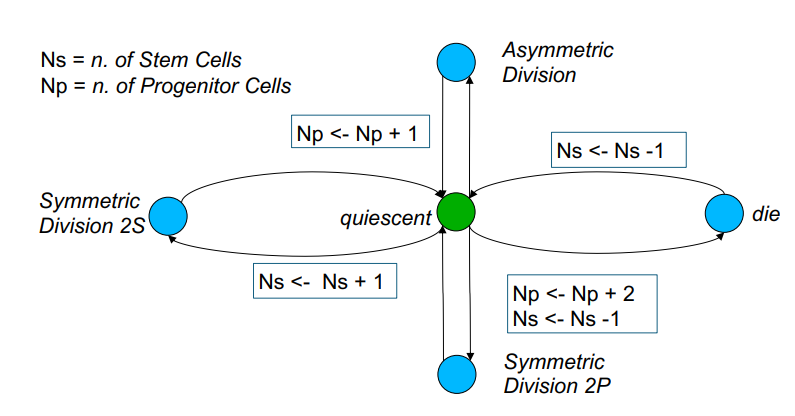
\includegraphics[width=.7\textwidth]{img/stemcellsFSA.png}
    \caption{Stem Cell Finite State Machine}
    \label{fig:stem_cell_fsm}
\end{figure}

In this example we don't consider the time. Time can be model considering an
exponential delay to the transition. Moreover, we can associate a different
probability to each transition, so we have a transition system (Markov Chain).
\section{Implementing a simulator}
In order to implement a simulator we need to define what means for us to run a
simulation. We can define a simulation as a sequence of events that can be
described by numerically solving a set of ODEs or by tracking the sequence of
events in a DES. This produce a \textbf{trace} of the simulation.

A trace is a sequence of vectors of values, where each vector represents the
state of the system at a given time. The trace can be used to analyze the
behavior of the system.

The engine of a simulator is essentially a loop where is body determines the
type of simulator we are using.
\subsection{Finite State Automata Simulator}
To implement a finite state automata simulator we need to define the following
elements:
\begin{itemize}
    \item \textbf{Specification}: first we need to define a set of finite
          automata, each represented by a matrix.
    \item \textbf{Engine}: check the set of all the enabled transitions from the
          current state and produce the next state.
    \item \textbf{Specification}: sources, computing units and sinks.
    \item \textbf{Trace}: a sequence of states.
\end{itemize}
